\documentclass[1p]{elsarticle_modified}
%\bibliographystyle{elsarticle-num}

%\usepackage[colorlinks]{hyperref}
%\usepackage{abbrmath_seonhwa} %\Abb, \Ascr, \Acal ,\Abf, \Afrak
\usepackage{amsfonts}
\usepackage{amssymb}
\usepackage{amsmath}
\usepackage{amsthm}
\usepackage{scalefnt}
\usepackage{amsbsy}
\usepackage{kotex}
\usepackage{caption}
\usepackage{subfig}
\usepackage{color}
\usepackage{graphicx}
\usepackage{xcolor} %% white, black, red, green, blue, cyan, magenta, yellow
\usepackage{float}
\usepackage{setspace}
\usepackage{hyperref}

\usepackage{tikz}
\usetikzlibrary{arrows}

\usepackage{multirow}
\usepackage{array} % fixed length table
\usepackage{hhline}

%%%%%%%%%%%%%%%%%%%%%
\makeatletter
\renewcommand*\env@matrix[1][\arraystretch]{%
	\edef\arraystretch{#1}%
	\hskip -\arraycolsep
	\let\@ifnextchar\new@ifnextchar
	\array{*\c@MaxMatrixCols c}}
\makeatother %https://tex.stackexchange.com/questions/14071/how-can-i-increase-the-line-spacing-in-a-matrix
%%%%%%%%%%%%%%%

\usepackage[normalem]{ulem}

\newcommand{\msout}[1]{\ifmmode\text{\sout{\ensuremath{#1}}}\else\sout{#1}\fi}
%SOURCE: \msout is \stkout macro in https://tex.stackexchange.com/questions/20609/strikeout-in-math-mode

\newcommand{\cancel}[1]{
	\ifmmode
	{\color{red}\msout{#1}}
	\else
	{\color{red}\sout{#1}}
	\fi
}

\newcommand{\add}[1]{
	{\color{blue}\uwave{#1}}
}

\newcommand{\replace}[2]{
	\ifmmode
	{\color{red}\msout{#1}}{\color{blue}\uwave{#2}}
	\else
	{\color{red}\sout{#1}}{\color{blue}\uwave{#2}}
	\fi
}

\newcommand{\Sol}{\mathcal{S}} %segment
\newcommand{\D}{D} %diagram
\newcommand{\A}{\mathcal{A}} %arc


%%%%%%%%%%%%%%%%%%%%%%%%%%%%%5 test

\def\sl{\operatorname{\textup{SL}}(2,\Cbb)}
\def\psl{\operatorname{\textup{PSL}}(2,\Cbb)}
\def\quan{\mkern 1mu \triangleright \mkern 1mu}

\theoremstyle{definition}
\newtheorem{thm}{Theorem}[section]
\newtheorem{prop}[thm]{Proposition}
\newtheorem{lem}[thm]{Lemma}
\newtheorem{ques}[thm]{Question}
\newtheorem{cor}[thm]{Corollary}
\newtheorem{defn}[thm]{Definition}
\newtheorem{exam}[thm]{Example}
\newtheorem{rmk}[thm]{Remark}
\newtheorem{alg}[thm]{Algorithm}

\newcommand{\I}{\sqrt{-1}}
\begin{document}

%\begin{frontmatter}
%
%\title{Boundary parabolic representations of knots up to 8 crossings}
%
%%% Group authors per affiliation:
%\author{Yunhi Cho} 
%\address{Department of Mathematics, University of Seoul, Seoul, Korea}
%\ead{yhcho@uos.ac.kr}
%
%
%\author{Seonhwa Kim} %\fnref{s_kim}}
%\address{Center for Geometry and Physics, Institute for Basic Science, Pohang, 37673, Korea}
%\ead{ryeona17@ibs.re.kr}
%
%\author{Hyuk Kim}
%\address{Department of Mathematical Sciences, Seoul National University, Seoul 08826, Korea}
%\ead{hyukkim@snu.ac.kr}
%
%\author{Seokbeom Yoon}
%\address{Department of Mathematical Sciences, Seoul National University, Seoul, 08826,  Korea}
%\ead{sbyoon15@snu.ac.kr}
%
%\begin{abstract}
%We find all boundary parabolic representation of knots up to 8 crossings.
%
%\end{abstract}
%\begin{keyword}
%    \MSC[2010] 57M25 
%\end{keyword}
%
%\end{frontmatter}

%\linenumbers
%\tableofcontents
%
\newcommand\colored[1]{\textcolor{white}{\rule[-0.35ex]{0.8em}{1.4ex}}\kern-0.8em\color{red} #1}%
%\newcommand\colored[1]{\textcolor{white}{ #1}\kern-2.17ex	\textcolor{white}{ #1}\kern-1.81ex	\textcolor{white}{ #1}\kern-2.15ex\color{red}#1	}

{\Large $\underline{12a_{0291}~(K12a_{0291})}$}

\setlength{\tabcolsep}{10pt}
\renewcommand{\arraystretch}{1.6}
\vspace{1cm}\begin{tabular}{m{100pt}>{\centering\arraybackslash}m{274pt}}
\multirow{5}{120pt}{
	\centering
	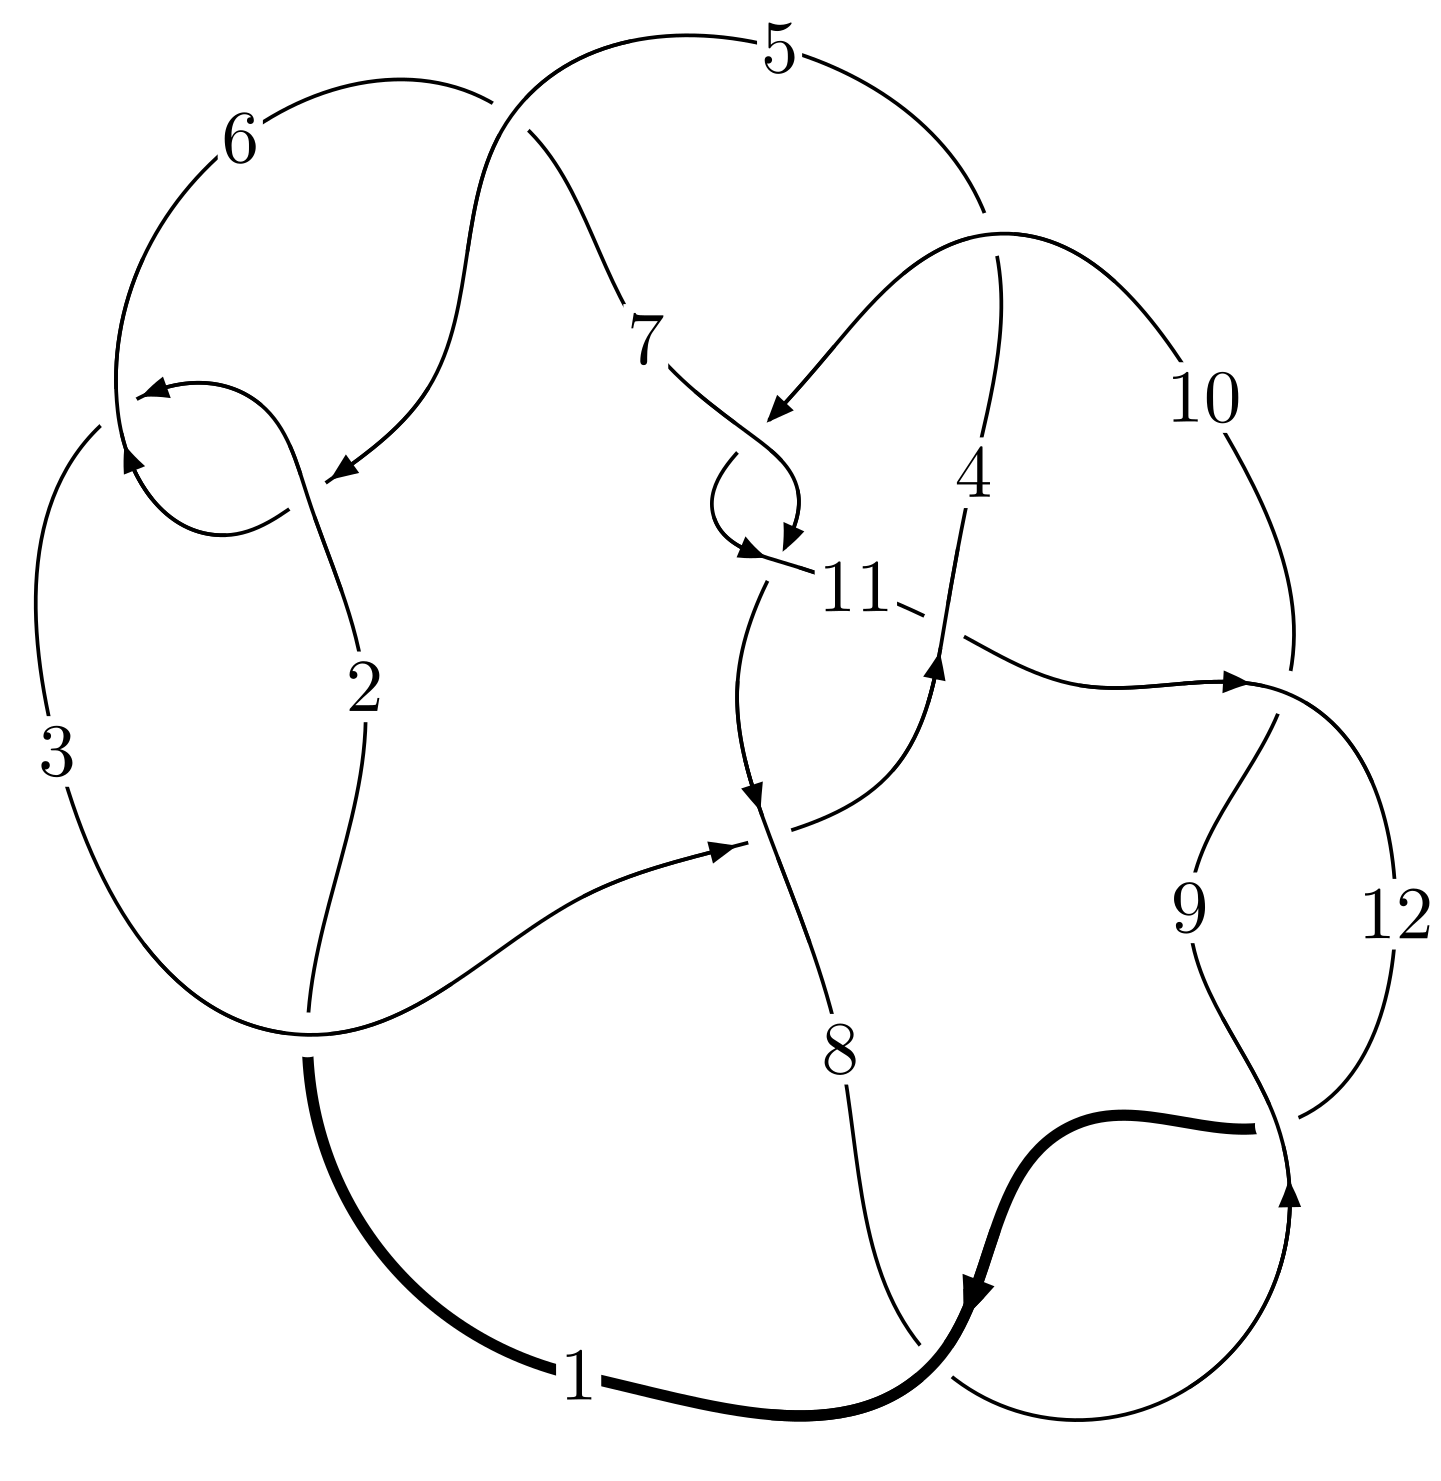
\includegraphics[width=112pt]{../../../GIT/diagram.site/Diagrams/png/1092_12a_0291.png}\\
\ \ \ A knot diagram\footnotemark}&
\allowdisplaybreaks
\textbf{Linearized knot diagam} \\
\cline{2-2}
 &
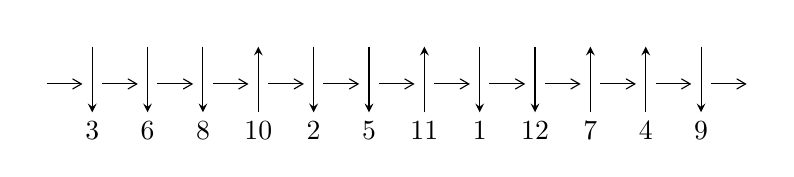
\begin{tikzpicture}[x=20pt, y=17pt]
	% nodes
	\node (C0) at (0, 0) {};
	\node (C1) at (1, 0) {};
	\node (C1U) at (1, +1) {};
	\node (C1D) at (1, -1) {3};

	\node (C2) at (2, 0) {};
	\node (C2U) at (2, +1) {};
	\node (C2D) at (2, -1) {6};

	\node (C3) at (3, 0) {};
	\node (C3U) at (3, +1) {};
	\node (C3D) at (3, -1) {8};

	\node (C4) at (4, 0) {};
	\node (C4U) at (4, +1) {};
	\node (C4D) at (4, -1) {10};

	\node (C5) at (5, 0) {};
	\node (C5U) at (5, +1) {};
	\node (C5D) at (5, -1) {2};

	\node (C6) at (6, 0) {};
	\node (C6U) at (6, +1) {};
	\node (C6D) at (6, -1) {5};

	\node (C7) at (7, 0) {};
	\node (C7U) at (7, +1) {};
	\node (C7D) at (7, -1) {11};

	\node (C8) at (8, 0) {};
	\node (C8U) at (8, +1) {};
	\node (C8D) at (8, -1) {1};

	\node (C9) at (9, 0) {};
	\node (C9U) at (9, +1) {};
	\node (C9D) at (9, -1) {12};

	\node (C10) at (10, 0) {};
	\node (C10U) at (10, +1) {};
	\node (C10D) at (10, -1) {7};

	\node (C11) at (11, 0) {};
	\node (C11U) at (11, +1) {};
	\node (C11D) at (11, -1) {4};

	\node (C12) at (12, 0) {};
	\node (C12U) at (12, +1) {};
	\node (C12D) at (12, -1) {9};
	\node (C13) at (13, 0) {};

	% arrows
	\draw[->,>={angle 60}]
	(C0) edge (C1) (C1) edge (C2) (C2) edge (C3) (C3) edge (C4) (C4) edge (C5) (C5) edge (C6) (C6) edge (C7) (C7) edge (C8) (C8) edge (C9) (C9) edge (C10) (C10) edge (C11) (C11) edge (C12) (C12) edge (C13) ;	\draw[->,>=stealth]
	(C1U) edge (C1D) (C2U) edge (C2D) (C3U) edge (C3D) (C4D) edge (C4U) (C5U) edge (C5D) (C6U) edge (C6D) (C7D) edge (C7U) (C8U) edge (C8D) (C9U) edge (C9D) (C10D) edge (C10U) (C11D) edge (C11U) (C12U) edge (C12D) ;
	\end{tikzpicture} \\
\hhline{~~} \\& 
\textbf{Solving Sequence} \\ \cline{2-2} 
 &
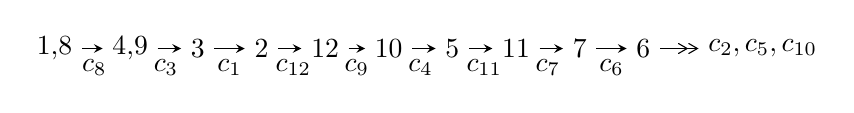
\begin{tikzpicture}[x=23pt, y=7pt]
	% node
	\node (A0) at (-1/8, 0) {1,8};
	\node (A1) at (17/16, 0) {4,9};
	\node (A2) at (17/8, 0) {3};
	\node (A3) at (25/8, 0) {2};
	\node (A4) at (33/8, 0) {12};
	\node (A5) at (41/8, 0) {10};
	\node (A6) at (49/8, 0) {5};
	\node (A7) at (57/8, 0) {11};
	\node (A8) at (65/8, 0) {7};
	\node (A9) at (73/8, 0) {6};
	\node (C1) at (1/2, -1) {$c_{8}$};
	\node (C2) at (13/8, -1) {$c_{3}$};
	\node (C3) at (21/8, -1) {$c_{1}$};
	\node (C4) at (29/8, -1) {$c_{12}$};
	\node (C5) at (37/8, -1) {$c_{9}$};
	\node (C6) at (45/8, -1) {$c_{4}$};
	\node (C7) at (53/8, -1) {$c_{11}$};
	\node (C8) at (61/8, -1) {$c_{7}$};
	\node (C9) at (69/8, -1) {$c_{6}$};
	\node (A10) at (11, 0) {$c_{2},c_{5},c_{10}$};

	% edge
	\draw[->,>=stealth]	
	(A0) edge (A1) (A1) edge (A2) (A2) edge (A3) (A3) edge (A4) (A4) edge (A5) (A5) edge (A6) (A6) edge (A7) (A7) edge (A8) (A8) edge (A9) ;
	\draw[->>,>={angle 60}]	
	(A9) edge (A10);
\end{tikzpicture} \\ 

\end{tabular} \\

\footnotetext{
The image of knot diagram is generated by the software ``\textbf{Draw programme}" developed by Andrew Bartholomew(\url{http://www.layer8.co.uk/maths/draw/index.htm\#Running-draw}), where we modified some parts for our purpose(\url{https://github.com/CATsTAILs/LinksPainter}).
}\phantom \\ \newline 
\centering \textbf{Ideals for irreducible components\footnotemark of $X_{\text{par}}$} 
 
\begin{align*}
I^u_{1}&=\langle 
-4.04111\times10^{126} u^{84}-1.47004\times10^{127} u^{83}+\cdots+7.92770\times10^{126} b+7.78808\times10^{126},\\
\phantom{I^u_{1}}&\phantom{= \langle  }-6.64112\times10^{126} u^{84}-2.58904\times10^{127} u^{83}+\cdots+7.92770\times10^{126} a-2.36197\times10^{127},\\
\phantom{I^u_{1}}&\phantom{= \langle  }u^{85}+4 u^{84}+\cdots+14 u+2\rangle \\
I^u_{2}&=\langle 
- a u+b,\;9 a^3-6 a^2 u+3 a^2-6 a+2 u-1,\;u^2- u+1\rangle \\
I^u_{3}&=\langle 
b+u+1,\;2 a-3 u-2,\;u^2+2\rangle \\
\\
I^v_{1}&=\langle 
a,\;b+1,\;v+1\rangle \\
\end{align*}
\raggedright * 4 irreducible components of $\dim_{\mathbb{C}}=0$, with total 94 representations.\\
\footnotetext{All coefficients of polynomials are rational numbers. But the coefficients are sometimes approximated in decimal forms when there is not enough margin.}
\newpage
\renewcommand{\arraystretch}{1}
\centering \section*{I. $I^u_{1}= \langle -4.04\times10^{126} u^{84}-1.47\times10^{127} u^{83}+\cdots+7.93\times10^{126} b+7.79\times10^{126},\;-6.64\times10^{126} u^{84}-2.59\times10^{127} u^{83}+\cdots+7.93\times10^{126} a-2.36\times10^{127},\;u^{85}+4 u^{84}+\cdots+14 u+2 \rangle$}
\flushleft \textbf{(i) Arc colorings}\\
\begin{tabular}{m{7pt} m{180pt} m{7pt} m{180pt} }
\flushright $a_{1}=$&$\begin{pmatrix}0\\u\end{pmatrix}$ \\
\flushright $a_{8}=$&$\begin{pmatrix}1\\0\end{pmatrix}$ \\
\flushright $a_{4}=$&$\begin{pmatrix}0.837711 u^{84}+3.26582 u^{83}+\cdots+23.0946 u+2.97939\\0.509746 u^{84}+1.85431 u^{83}+\cdots+2.63027 u-0.982389\end{pmatrix}$ \\
\flushright $a_{9}=$&$\begin{pmatrix}1\\u^2\end{pmatrix}$ \\
\flushright $a_{3}=$&$\begin{pmatrix}1.34746 u^{84}+5.12014 u^{83}+\cdots+25.7249 u+1.99700\\0.509746 u^{84}+1.85431 u^{83}+\cdots+2.63027 u-0.982389\end{pmatrix}$ \\
\flushright $a_{2}=$&$\begin{pmatrix}-1.26472 u^{84}-6.06172 u^{83}+\cdots-91.5000 u-16.8602\\0.598452 u^{84}+2.02176 u^{83}+\cdots+4.76229 u-0.278731\end{pmatrix}$ \\
\flushright $a_{12}=$&$\begin{pmatrix}u\\u^3+u\end{pmatrix}$ \\
\flushright $a_{10}=$&$\begin{pmatrix}u^2+1\\u^4+2 u^2\end{pmatrix}$ \\
\flushright $a_{5}=$&$\begin{pmatrix}1.72649 u^{84}+6.50029 u^{83}+\cdots+34.3325 u+3.23940\\0.519117 u^{84}+2.00224 u^{83}+\cdots+9.39854 u+0.520508\end{pmatrix}$ \\
\flushright $a_{11}=$&$\begin{pmatrix}-2.50474 u^{84}-10.2416 u^{83}+\cdots-93.6888 u-15.3979\\0.592317 u^{84}+2.10401 u^{83}+\cdots+9.22146 u+0.356710\end{pmatrix}$ \\
\flushright $a_{7}=$&$\begin{pmatrix}-2.36646 u^{84}-9.65905 u^{83}+\cdots-94.7830 u-15.3092\\0.509534 u^{84}+1.79876 u^{83}+\cdots+6.34356 u+0.475093\end{pmatrix}$ \\
\flushright $a_{6}=$&$\begin{pmatrix}0.0492125 u^{84}+0.616005 u^{83}+\cdots+18.7360 u+3.81121\\-0.258472 u^{84}-0.807102 u^{83}+\cdots+0.539727 u+0.813419\end{pmatrix}$\\&\end{tabular}
\flushleft \textbf{(ii) Obstruction class $= -1$}\\~\\
\flushleft \textbf{(iii) Cusp Shapes $= -1.70495 u^{84}-5.18172 u^{83}+\cdots+36.7845 u+15.0874$}\\~\\
\newpage\renewcommand{\arraystretch}{1}
\flushleft \textbf{(iv) u-Polynomials at the component}\newline \\
\begin{tabular}{m{50pt}|m{274pt}}
Crossings & \hspace{64pt}u-Polynomials at each crossing \\
\hline $$\begin{aligned}c_{1},c_{6}\end{aligned}$$&$\begin{aligned}
&u^{85}+24 u^{84}+\cdots+97 u+81
\end{aligned}$\\
\hline $$\begin{aligned}c_{2},c_{5}\end{aligned}$$&$\begin{aligned}
&u^{85}+6 u^{84}+\cdots+23 u+9
\end{aligned}$\\
\hline $$\begin{aligned}c_{3}\end{aligned}$$&$\begin{aligned}
&27(27 u^{85}-153 u^{84}+\cdots-2.29371\times10^{8} u+3.37805\times10^{7})
\end{aligned}$\\
\hline $$\begin{aligned}c_{4}\end{aligned}$$&$\begin{aligned}
&27(27 u^{85}+288 u^{84}+\cdots-8003245 u+2090863)
\end{aligned}$\\
\hline $$\begin{aligned}c_{7},c_{10}\end{aligned}$$&$\begin{aligned}
&u^{85}-5 u^{84}+\cdots+18 u+3
\end{aligned}$\\
\hline $$\begin{aligned}c_{8},c_{9},c_{12}\end{aligned}$$&$\begin{aligned}
&u^{85}-4 u^{84}+\cdots+14 u-2
\end{aligned}$\\
\hline $$\begin{aligned}c_{11}\end{aligned}$$&$\begin{aligned}
&u^{85}-4 u^{84}+\cdots-33696 u+5184
\end{aligned}$\\
\hline
\end{tabular}\\~\\
\newpage\renewcommand{\arraystretch}{1}
\flushleft \textbf{(v) Riley Polynomials at the component}\newline \\
\begin{tabular}{m{50pt}|m{274pt}}
Crossings & \hspace{64pt}Riley Polynomials at each crossing \\
\hline $$\begin{aligned}c_{1},c_{6}\end{aligned}$$&$\begin{aligned}
&y^{85}+80 y^{84}+\cdots+824593 y-6561
\end{aligned}$\\
\hline $$\begin{aligned}c_{2},c_{5}\end{aligned}$$&$\begin{aligned}
&y^{85}-24 y^{84}+\cdots+97 y-81
\end{aligned}$\\
\hline $$\begin{aligned}c_{3}\end{aligned}$$&$\begin{aligned}
&729(729 y^{85}+35559 y^{84}+\cdots-6.28776\times10^{15} y-1.14112\times10^{15})
\end{aligned}$\\
\hline $$\begin{aligned}c_{4}\end{aligned}$$&$\begin{aligned}
&729\\
&\cdot(729 y^{85}-51192 y^{84}+\cdots+103418130379289 y-4371708084769)
\end{aligned}$\\
\hline $$\begin{aligned}c_{7},c_{10}\end{aligned}$$&$\begin{aligned}
&y^{85}-59 y^{84}+\cdots+966 y-9
\end{aligned}$\\
\hline $$\begin{aligned}c_{8},c_{9},c_{12}\end{aligned}$$&$\begin{aligned}
&y^{85}+88 y^{84}+\cdots-52 y-4
\end{aligned}$\\
\hline $$\begin{aligned}c_{11}\end{aligned}$$&$\begin{aligned}
&y^{85}-38 y^{84}+\cdots+338162688 y-26873856
\end{aligned}$\\
\hline
\end{tabular}\\~\\
\newpage\flushleft \textbf{(vi) Complex Volumes and Cusp Shapes}
$$\begin{array}{c|c|c}  
\text{Solutions to }I^u_{1}& \I (\text{vol} + \sqrt{-1}CS) & \text{Cusp shape}\\
 \hline 
\begin{aligned}
u &= -0.802781 + 0.666760 I \\
a &= \phantom{-}0.444154 + 0.389043 I \\
b &= \phantom{-}0.54776 - 1.33558 I\end{aligned}
 & \phantom{-}9.35665 + 6.36583 I & \phantom{-0.000000 } 0 \\ \hline\begin{aligned}
u &= -0.802781 - 0.666760 I \\
a &= \phantom{-}0.444154 - 0.389043 I \\
b &= \phantom{-}0.54776 + 1.33558 I\end{aligned}
 & \phantom{-}9.35665 - 6.36583 I & \phantom{-0.000000 } 0 \\ \hline\begin{aligned}
u &= -0.840661 + 0.625642 I \\
a &= -0.546357 - 0.360547 I \\
b &= -0.64122 + 1.40506 I\end{aligned}
 & \phantom{-}8.7128 + 12.6729 I & \phantom{-0.000000 } 0 \\ \hline\begin{aligned}
u &= -0.840661 - 0.625642 I \\
a &= -0.546357 + 0.360547 I \\
b &= -0.64122 - 1.40506 I\end{aligned}
 & \phantom{-}8.7128 - 12.6729 I & \phantom{-0.000000 } 0 \\ \hline\begin{aligned}
u &= -0.933727 + 0.500289 I \\
a &= -0.710871 + 0.140901 I \\
b &= \phantom{-}0.067748 + 1.068420 I\end{aligned}
 & \phantom{-}8.75934 - 0.64306 I & \phantom{-0.000000 } 0 \\ \hline\begin{aligned}
u &= -0.933727 - 0.500289 I \\
a &= -0.710871 - 0.140901 I \\
b &= \phantom{-}0.067748 - 1.068420 I\end{aligned}
 & \phantom{-}8.75934 + 0.64306 I & \phantom{-0.000000 } 0 \\ \hline\begin{aligned}
u &= \phantom{-}0.099564 + 1.061390 I \\
a &= \phantom{-}0.055284 - 0.183938 I \\
b &= -0.804734 - 0.275552 I\end{aligned}
 & \phantom{-}1.46155 - 0.12863 I & \phantom{-0.000000 } 0 \\ \hline\begin{aligned}
u &= \phantom{-}0.099564 - 1.061390 I \\
a &= \phantom{-}0.055284 + 0.183938 I \\
b &= -0.804734 + 0.275552 I\end{aligned}
 & \phantom{-}1.46155 + 0.12863 I & \phantom{-0.000000 } 0 \\ \hline\begin{aligned}
u &= -0.922718 + 0.564249 I \\
a &= \phantom{-}0.711488 - 0.159783 I \\
b &= -0.149669 - 1.177890 I\end{aligned}
 & \phantom{-}8.44674 - 6.85650 I & \phantom{-0.000000 } 0 \\ \hline\begin{aligned}
u &= -0.922718 - 0.564249 I \\
a &= \phantom{-}0.711488 + 0.159783 I \\
b &= -0.149669 + 1.177890 I\end{aligned}
 & \phantom{-}8.44674 + 6.85650 I & \phantom{-0.000000 } 0\\
 \hline 
 \end{array}$$\newpage$$\begin{array}{c|c|c}  
\text{Solutions to }I^u_{1}& \I (\text{vol} + \sqrt{-1}CS) & \text{Cusp shape}\\
 \hline 
\begin{aligned}
u &= \phantom{-}0.593150 + 0.919610 I \\
a &= -0.1315520 - 0.0150511 I \\
b &= \phantom{-}0.268708 - 0.398741 I\end{aligned}
 & -0.92845 - 1.82818 I & \phantom{-0.000000 } 0 \\ \hline\begin{aligned}
u &= \phantom{-}0.593150 - 0.919610 I \\
a &= -0.1315520 + 0.0150511 I \\
b &= \phantom{-}0.268708 + 0.398741 I\end{aligned}
 & -0.92845 + 1.82818 I & \phantom{-0.000000 } 0 \\ \hline\begin{aligned}
u &= \phantom{-}0.951786 + 0.650510 I \\
a &= \phantom{-}0.486994 - 0.119384 I \\
b &= \phantom{-}0.391324 + 1.066140 I\end{aligned}
 & \phantom{-}3.74898 - 6.20791 I & \phantom{-0.000000 } 0 \\ \hline\begin{aligned}
u &= \phantom{-}0.951786 - 0.650510 I \\
a &= \phantom{-}0.486994 + 0.119384 I \\
b &= \phantom{-}0.391324 - 1.066140 I\end{aligned}
 & \phantom{-}3.74898 + 6.20791 I & \phantom{-0.000000 } 0 \\ \hline\begin{aligned}
u &= \phantom{-}0.925364 + 0.717550 I \\
a &= -0.440303 + 0.082121 I \\
b &= -0.238296 - 1.072720 I\end{aligned}
 & \phantom{-}3.93970 - 0.17528 I & \phantom{-0.000000 } 0 \\ \hline\begin{aligned}
u &= \phantom{-}0.925364 - 0.717550 I \\
a &= -0.440303 - 0.082121 I \\
b &= -0.238296 + 1.072720 I\end{aligned}
 & \phantom{-}3.93970 + 0.17528 I & \phantom{-0.000000 } 0 \\ \hline\begin{aligned}
u &= \phantom{-}0.727828 + 0.390455 I \\
a &= \phantom{-}0.449726 - 0.488595 I \\
b &= \phantom{-}0.525964 + 0.518969 I\end{aligned}
 & -2.30865 - 2.94104 I & \phantom{-0.000000 } 0 \\ \hline\begin{aligned}
u &= \phantom{-}0.727828 - 0.390455 I \\
a &= \phantom{-}0.449726 + 0.488595 I \\
b &= \phantom{-}0.525964 - 0.518969 I\end{aligned}
 & -2.30865 + 2.94104 I & \phantom{-0.000000 } 0 \\ \hline\begin{aligned}
u &= \phantom{-}0.325597 + 1.142700 I \\
a &= \phantom{-}0.0448468 - 0.0603608 I \\
b &= \phantom{-}0.789387 + 0.068143 I\end{aligned}
 & \phantom{-}1.61955 - 4.56441 I & \phantom{-0.000000 } 0 \\ \hline\begin{aligned}
u &= \phantom{-}0.325597 - 1.142700 I \\
a &= \phantom{-}0.0448468 + 0.0603608 I \\
b &= \phantom{-}0.789387 - 0.068143 I\end{aligned}
 & \phantom{-}1.61955 + 4.56441 I & \phantom{-0.000000 } 0\\
 \hline 
 \end{array}$$\newpage$$\begin{array}{c|c|c}  
\text{Solutions to }I^u_{1}& \I (\text{vol} + \sqrt{-1}CS) & \text{Cusp shape}\\
 \hline 
\begin{aligned}
u &= -0.567914 + 0.571899 I \\
a &= \phantom{-}0.604728 - 0.178179 I \\
b &= -0.644834 - 0.904739 I\end{aligned}
 & \phantom{-}1.38177 - 3.51715 I & \phantom{-0.000000 } 0 \\ \hline\begin{aligned}
u &= -0.567914 - 0.571899 I \\
a &= \phantom{-}0.604728 + 0.178179 I \\
b &= -0.644834 + 0.904739 I\end{aligned}
 & \phantom{-}1.38177 + 3.51715 I & \phantom{-0.000000 } 0 \\ \hline\begin{aligned}
u &= -0.641156 + 0.471692 I \\
a &= -0.731557 - 0.940849 I \\
b &= -0.817818 + 0.973867 I\end{aligned}
 & \phantom{-}1.07426 + 7.71240 I & \phantom{-0.000000 } 0 \\ \hline\begin{aligned}
u &= -0.641156 - 0.471692 I \\
a &= -0.731557 + 0.940849 I \\
b &= -0.817818 - 0.973867 I\end{aligned}
 & \phantom{-}1.07426 - 7.71240 I & \phantom{-0.000000 } 0 \\ \hline\begin{aligned}
u &= -0.460489 + 0.587516 I \\
a &= \phantom{-}0.051839 + 1.283270 I \\
b &= \phantom{-}0.590387 - 0.821616 I\end{aligned}
 & \phantom{-}4.12766 + 3.84400 I & \phantom{-}3.48726 - 5.71525 I \\ \hline\begin{aligned}
u &= -0.460489 - 0.587516 I \\
a &= \phantom{-}0.051839 - 1.283270 I \\
b &= \phantom{-}0.590387 + 0.821616 I\end{aligned}
 & \phantom{-}4.12766 - 3.84400 I & \phantom{-}3.48726 + 5.71525 I \\ \hline\begin{aligned}
u &= \phantom{-}0.167924 + 0.707939 I \\
a &= -2.22545 + 0.77882 I \\
b &= \phantom{-}0.356883 - 0.967640 I\end{aligned}
 & \phantom{-}7.83381 + 0.86043 I & \phantom{-}5.30165 + 0. I\phantom{ +0.000000I} \\ \hline\begin{aligned}
u &= \phantom{-}0.167924 - 0.707939 I \\
a &= -2.22545 - 0.77882 I \\
b &= \phantom{-}0.356883 + 0.967640 I\end{aligned}
 & \phantom{-}7.83381 - 0.86043 I & \phantom{-}5.30165 + 0. I\phantom{ +0.000000I} \\ \hline\begin{aligned}
u &= \phantom{-}0.289362 + 0.616253 I \\
a &= \phantom{-}2.51494 - 0.45923 I \\
b &= -0.143489 + 0.984157 I\end{aligned}
 & \phantom{-}7.12241 - 5.37900 I & \phantom{-}3.62062 + 6.29663 I \\ \hline\begin{aligned}
u &= \phantom{-}0.289362 - 0.616253 I \\
a &= \phantom{-}2.51494 + 0.45923 I \\
b &= -0.143489 - 0.984157 I\end{aligned}
 & \phantom{-}7.12241 + 5.37900 I & \phantom{-}3.62062 - 6.29663 I\\
 \hline 
 \end{array}$$\newpage$$\begin{array}{c|c|c}  
\text{Solutions to }I^u_{1}& \I (\text{vol} + \sqrt{-1}CS) & \text{Cusp shape}\\
 \hline 
\begin{aligned}
u &= -0.585513 + 0.213693 I \\
a &= -0.594955 + 0.071624 I \\
b &= \phantom{-}0.580910 + 0.428079 I\end{aligned}
 & \phantom{-}3.00184 - 0.43149 I & \phantom{-}1.31859 - 2.45780 I \\ \hline\begin{aligned}
u &= -0.585513 - 0.213693 I \\
a &= -0.594955 - 0.071624 I \\
b &= \phantom{-}0.580910 - 0.428079 I\end{aligned}
 & \phantom{-}3.00184 + 0.43149 I & \phantom{-}1.31859 + 2.45780 I \\ \hline\begin{aligned}
u &= -0.180672 + 1.380910 I \\
a &= -1.23127 - 0.96960 I \\
b &= \phantom{-}0.679911 + 0.815725 I\end{aligned}
 & \phantom{-}7.94632 + 2.41671 I & \phantom{-0.000000 } 0 \\ \hline\begin{aligned}
u &= -0.180672 - 1.380910 I \\
a &= -1.23127 + 0.96960 I \\
b &= \phantom{-}0.679911 - 0.815725 I\end{aligned}
 & \phantom{-}7.94632 - 2.41671 I & \phantom{-0.000000 } 0 \\ \hline\begin{aligned}
u &= \phantom{-}0.050758 + 1.403220 I \\
a &= \phantom{-}0.14372 - 1.51124 I \\
b &= -0.444961 + 0.783429 I\end{aligned}
 & \phantom{-}2.89071 - 0.02350 I & \phantom{-0.000000 } 0 \\ \hline\begin{aligned}
u &= \phantom{-}0.050758 - 1.403220 I \\
a &= \phantom{-}0.14372 + 1.51124 I \\
b &= -0.444961 - 0.783429 I\end{aligned}
 & \phantom{-}2.89071 + 0.02350 I & \phantom{-0.000000 } 0 \\ \hline\begin{aligned}
u &= \phantom{-}0.027731 + 1.406400 I \\
a &= -3.96077 + 1.85576 I \\
b &= \phantom{-}4.01105 - 2.17001 I\end{aligned}
 & \phantom{-}5.66382 - 0.10661 I & \phantom{-0.000000 } 0 \\ \hline\begin{aligned}
u &= \phantom{-}0.027731 - 1.406400 I \\
a &= -3.96077 - 1.85576 I \\
b &= \phantom{-}4.01105 + 2.17001 I\end{aligned}
 & \phantom{-}5.66382 + 0.10661 I & \phantom{-0.000000 } 0 \\ \hline\begin{aligned}
u &= \phantom{-}0.332326 + 0.422048 I \\
a &= \phantom{-}0.224263 + 0.635046 I \\
b &= -0.268723 - 0.452263 I\end{aligned}
 & -0.065957 - 1.057420 I & -1.21607 + 6.29792 I \\ \hline\begin{aligned}
u &= \phantom{-}0.332326 - 0.422048 I \\
a &= \phantom{-}0.224263 - 0.635046 I \\
b &= -0.268723 + 0.452263 I\end{aligned}
 & -0.065957 + 1.057420 I & -1.21607 - 6.29792 I\\
 \hline 
 \end{array}$$\newpage$$\begin{array}{c|c|c}  
\text{Solutions to }I^u_{1}& \I (\text{vol} + \sqrt{-1}CS) & \text{Cusp shape}\\
 \hline 
\begin{aligned}
u &= \phantom{-}0.514945 + 0.052028 I \\
a &= \phantom{-}0.63587 - 1.41127 I \\
b &= \phantom{-}0.326392 + 0.017339 I\end{aligned}
 & -1.57079 + 1.46950 I & -9.77061 - 4.07897 I \\ \hline\begin{aligned}
u &= \phantom{-}0.514945 - 0.052028 I \\
a &= \phantom{-}0.63587 + 1.41127 I \\
b &= \phantom{-}0.326392 - 0.017339 I\end{aligned}
 & -1.57079 - 1.46950 I & -9.77061 + 4.07897 I \\ \hline\begin{aligned}
u &= \phantom{-}0.21356 + 1.47274 I \\
a &= \phantom{-}0.10247 - 1.46449 I \\
b &= \phantom{-}0.452591 + 0.938205 I\end{aligned}
 & \phantom{-}3.73750 - 6.24800 I & \phantom{-0.000000 } 0 \\ \hline\begin{aligned}
u &= \phantom{-}0.21356 - 1.47274 I \\
a &= \phantom{-}0.10247 + 1.46449 I \\
b &= \phantom{-}0.452591 - 0.938205 I\end{aligned}
 & \phantom{-}3.73750 + 6.24800 I & \phantom{-0.000000 } 0 \\ \hline\begin{aligned}
u &= -0.06407 + 1.49452 I \\
a &= \phantom{-}0.51861 - 2.01899 I \\
b &= -0.171203 + 0.869357 I\end{aligned}
 & \phantom{-}6.16680 + 1.75465 I & \phantom{-0.000000 } 0 \\ \hline\begin{aligned}
u &= -0.06407 - 1.49452 I \\
a &= \phantom{-}0.51861 + 2.01899 I \\
b &= -0.171203 - 0.869357 I\end{aligned}
 & \phantom{-}6.16680 - 1.75465 I & \phantom{-0.000000 } 0 \\ \hline\begin{aligned}
u &= -0.05194 + 1.49750 I \\
a &= \phantom{-}0.75573 - 1.32650 I \\
b &= -1.77024 + 1.16248 I\end{aligned}
 & \phantom{-}9.30893 + 4.57642 I & \phantom{-0.000000 } 0 \\ \hline\begin{aligned}
u &= -0.05194 - 1.49750 I \\
a &= \phantom{-}0.75573 + 1.32650 I \\
b &= -1.77024 - 1.16248 I\end{aligned}
 & \phantom{-}9.30893 - 4.57642 I & \phantom{-0.000000 } 0 \\ \hline\begin{aligned}
u &= -0.01980 + 1.50512 I \\
a &= -0.87950 + 1.48472 I \\
b &= \phantom{-}1.77677 - 1.49662 I\end{aligned}
 & \phantom{-}9.72935 - 1.45679 I & \phantom{-0.000000 } 0 \\ \hline\begin{aligned}
u &= -0.01980 - 1.50512 I \\
a &= -0.87950 - 1.48472 I \\
b &= \phantom{-}1.77677 + 1.49662 I\end{aligned}
 & \phantom{-}9.72935 + 1.45679 I & \phantom{-0.000000 } 0\\
 \hline 
 \end{array}$$\newpage$$\begin{array}{c|c|c}  
\text{Solutions to }I^u_{1}& \I (\text{vol} + \sqrt{-1}CS) & \text{Cusp shape}\\
 \hline 
\begin{aligned}
u &= \phantom{-}0.10823 + 1.51105 I \\
a &= -0.04805 + 1.53309 I \\
b &= -0.088616 - 1.270120 I\end{aligned}
 & \phantom{-}6.46358 - 2.67802 I & \phantom{-0.000000 } 0 \\ \hline\begin{aligned}
u &= \phantom{-}0.10823 - 1.51105 I \\
a &= -0.04805 - 1.53309 I \\
b &= -0.088616 + 1.270120 I\end{aligned}
 & \phantom{-}6.46358 + 2.67802 I & \phantom{-0.000000 } 0 \\ \hline\begin{aligned}
u &= -0.19892 + 1.50982 I \\
a &= \phantom{-}0.04052 - 1.96137 I \\
b &= -0.74982 + 1.25661 I\end{aligned}
 & \phantom{-}7.58189 + 10.73300 I & \phantom{-0.000000 } 0 \\ \hline\begin{aligned}
u &= -0.19892 - 1.50982 I \\
a &= \phantom{-}0.04052 + 1.96137 I \\
b &= -0.74982 - 1.25661 I\end{aligned}
 & \phantom{-}7.58189 - 10.73300 I & \phantom{-0.000000 } 0 \\ \hline\begin{aligned}
u &= -0.09406 + 1.52146 I \\
a &= \phantom{-}0.60512 + 1.61508 I \\
b &= -0.19813 - 1.69091 I\end{aligned}
 & \phantom{-}8.39441 - 1.40303 I & \phantom{-0.000000 } 0 \\ \hline\begin{aligned}
u &= -0.09406 - 1.52146 I \\
a &= \phantom{-}0.60512 - 1.61508 I \\
b &= -0.19813 + 1.69091 I\end{aligned}
 & \phantom{-}8.39441 + 1.40303 I & \phantom{-0.000000 } 0 \\ \hline\begin{aligned}
u &= -0.176623 + 0.430115 I \\
a &= \phantom{-}1.88458 - 0.21008 I \\
b &= \phantom{-}0.469587 - 1.100450 I\end{aligned}
 & \phantom{-}3.24208 - 1.99205 I & \phantom{-}1.86195 + 5.62347 I \\ \hline\begin{aligned}
u &= -0.176623 - 0.430115 I \\
a &= \phantom{-}1.88458 + 0.21008 I \\
b &= \phantom{-}0.469587 + 1.100450 I\end{aligned}
 & \phantom{-}3.24208 + 1.99205 I & \phantom{-}1.86195 - 5.62347 I \\ \hline\begin{aligned}
u &= -0.246167 + 0.375896 I \\
a &= -2.13263 + 0.10858 I \\
b &= -0.714174 + 0.978375 I\end{aligned}
 & \phantom{-}3.01363 + 3.62679 I & \phantom{-}0.237626 - 0.197969 I \\ \hline\begin{aligned}
u &= -0.246167 - 0.375896 I \\
a &= -2.13263 - 0.10858 I \\
b &= -0.714174 - 0.978375 I\end{aligned}
 & \phantom{-}3.01363 - 3.62679 I & \phantom{-}0.237626 + 0.197969 I\\
 \hline 
 \end{array}$$\newpage$$\begin{array}{c|c|c}  
\text{Solutions to }I^u_{1}& \I (\text{vol} + \sqrt{-1}CS) & \text{Cusp shape}\\
 \hline 
\begin{aligned}
u &= -0.13362 + 1.54561 I \\
a &= -0.19237 + 1.85508 I \\
b &= \phantom{-}0.374741 - 1.266880 I\end{aligned}
 & \phantom{-}11.23470 + 5.99704 I & \phantom{-0.000000 } 0 \\ \hline\begin{aligned}
u &= -0.13362 - 1.54561 I \\
a &= -0.19237 - 1.85508 I \\
b &= \phantom{-}0.374741 + 1.266880 I\end{aligned}
 & \phantom{-}11.23470 - 5.99704 I & \phantom{-0.000000 } 0 \\ \hline\begin{aligned}
u &= \phantom{-}0.07557 + 1.55121 I \\
a &= \phantom{-}0.653295 - 1.130100 I \\
b &= \phantom{-}0.576031 + 0.900387 I\end{aligned}
 & \phantom{-}14.3920 - 6.6683 I & \phantom{-0.000000 } 0 \\ \hline\begin{aligned}
u &= \phantom{-}0.07557 - 1.55121 I \\
a &= \phantom{-}0.653295 + 1.130100 I \\
b &= \phantom{-}0.576031 - 0.900387 I\end{aligned}
 & \phantom{-}14.3920 + 6.6683 I & \phantom{-0.000000 } 0 \\ \hline\begin{aligned}
u &= \phantom{-}0.440029 + 0.047676 I \\
a &= \phantom{-}0.040169 - 0.742148 I \\
b &= \phantom{-}0.00599 - 2.44474 I\end{aligned}
 & \phantom{-}5.42251 + 2.96044 I & -11.24832 - 0.49298 I \\ \hline\begin{aligned}
u &= \phantom{-}0.440029 - 0.047676 I \\
a &= \phantom{-}0.040169 + 0.742148 I \\
b &= \phantom{-}0.00599 + 2.44474 I\end{aligned}
 & \phantom{-}5.42251 - 2.96044 I & -11.24832 + 0.49298 I \\ \hline\begin{aligned}
u &= \phantom{-}0.03178 + 1.56804 I \\
a &= -0.58241 + 1.33803 I \\
b &= -0.417899 - 1.034010 I\end{aligned}
 & \phantom{-}15.4735 + 0.2256 I & \phantom{-0.000000 } 0 \\ \hline\begin{aligned}
u &= \phantom{-}0.03178 - 1.56804 I \\
a &= -0.58241 - 1.33803 I \\
b &= -0.417899 + 1.034010 I\end{aligned}
 & \phantom{-}15.4735 - 0.2256 I & \phantom{-0.000000 } 0 \\ \hline\begin{aligned}
u &= -0.257488 + 0.337643 I \\
a &= -0.37428 - 3.54840 I \\
b &= -0.584493 + 0.525668 I\end{aligned}
 & -0.025237 + 0.681729 I & \phantom{-}0.12938 - 10.39624 I \\ \hline\begin{aligned}
u &= -0.257488 - 0.337643 I \\
a &= -0.37428 + 3.54840 I \\
b &= -0.584493 - 0.525668 I\end{aligned}
 & -0.025237 - 0.681729 I & \phantom{-}0.12938 + 10.39624 I\\
 \hline 
 \end{array}$$\newpage$$\begin{array}{c|c|c}  
\text{Solutions to }I^u_{1}& \I (\text{vol} + \sqrt{-1}CS) & \text{Cusp shape}\\
 \hline 
\begin{aligned}
u &= -0.28292 + 1.58422 I \\
a &= -0.13616 - 1.84338 I \\
b &= -0.95678 + 1.78318 I\end{aligned}
 & \phantom{-}15.9618 + 16.8256 I & \phantom{-0.000000 } 0 \\ \hline\begin{aligned}
u &= -0.28292 - 1.58422 I \\
a &= -0.13616 + 1.84338 I \\
b &= -0.95678 - 1.78318 I\end{aligned}
 & \phantom{-}15.9618 - 16.8256 I & \phantom{-0.000000 } 0 \\ \hline\begin{aligned}
u &= -0.25995 + 1.59435 I \\
a &= \phantom{-}0.10124 + 1.81756 I \\
b &= \phantom{-}0.82984 - 1.77590 I\end{aligned}
 & \phantom{-}16.8148 + 10.3036 I & \phantom{-0.000000 } 0 \\ \hline\begin{aligned}
u &= -0.25995 - 1.59435 I \\
a &= \phantom{-}0.10124 - 1.81756 I \\
b &= \phantom{-}0.82984 + 1.77590 I\end{aligned}
 & \phantom{-}16.8148 - 10.3036 I & \phantom{-0.000000 } 0 \\ \hline\begin{aligned}
u &= -0.34489 + 1.59776 I \\
a &= -0.440689 - 0.952425 I \\
b &= -0.512257 + 1.080120 I\end{aligned}
 & \phantom{-}15.6088 + 4.1683 I & \phantom{-0.000000 } 0 \\ \hline\begin{aligned}
u &= -0.34489 - 1.59776 I \\
a &= -0.440689 + 0.952425 I \\
b &= -0.512257 - 1.080120 I\end{aligned}
 & \phantom{-}15.6088 - 4.1683 I & \phantom{-0.000000 } 0 \\ \hline\begin{aligned}
u &= \phantom{-}0.29557 + 1.61174 I \\
a &= \phantom{-}0.065113 - 1.385510 I \\
b &= \phantom{-}0.93022 + 1.37397 I\end{aligned}
 & \phantom{-}11.2264 - 10.7656 I & \phantom{-0.000000 } 0 \\ \hline\begin{aligned}
u &= \phantom{-}0.29557 - 1.61174 I \\
a &= \phantom{-}0.065113 + 1.385510 I \\
b &= \phantom{-}0.93022 - 1.37397 I\end{aligned}
 & \phantom{-}11.2264 + 10.7656 I & \phantom{-0.000000 } 0 \\ \hline\begin{aligned}
u &= \phantom{-}0.26193 + 1.62559 I \\
a &= -0.048549 + 1.391250 I \\
b &= -0.81923 - 1.46077 I\end{aligned}
 & \phantom{-}11.77100 - 4.49005 I & \phantom{-0.000000 } 0 \\ \hline\begin{aligned}
u &= \phantom{-}0.26193 - 1.62559 I \\
a &= -0.048549 - 1.391250 I \\
b &= -0.81923 + 1.46077 I\end{aligned}
 & \phantom{-}11.77100 + 4.49005 I & \phantom{-0.000000 } 0\\
 \hline 
 \end{array}$$\newpage$$\begin{array}{c|c|c}  
\text{Solutions to }I^u_{1}& \I (\text{vol} + \sqrt{-1}CS) & \text{Cusp shape}\\
 \hline 
\begin{aligned}
u &= -0.31266 + 1.62469 I \\
a &= \phantom{-}0.420595 + 1.013950 I \\
b &= \phantom{-}0.488380 - 1.232340 I\end{aligned}
 & \phantom{-}15.6769 - 2.1737 I & \phantom{-0.000000 } 0 \\ \hline\begin{aligned}
u &= -0.31266 - 1.62469 I \\
a &= \phantom{-}0.420595 - 1.013950 I \\
b &= \phantom{-}0.488380 + 1.232340 I\end{aligned}
 & \phantom{-}15.6769 + 2.1737 I & \phantom{-0.000000 } 0 \\ \hline\begin{aligned}
u &= \phantom{-}0.047792 + 0.283678 I \\
a &= \phantom{-}0.434605 - 0.380197 I \\
b &= -0.75550 - 1.74214 I\end{aligned}
 & \phantom{-}0.336343 + 0.330613 I & \phantom{-}14.7201 + 7.4977 I \\ \hline\begin{aligned}
u &= \phantom{-}0.047792 - 0.283678 I \\
a &= \phantom{-}0.434605 + 0.380197 I \\
b &= -0.75550 + 1.74214 I\end{aligned}
 & \phantom{-}0.336343 - 0.330613 I & \phantom{-}14.7201 - 7.4977 I \\ \hline\begin{aligned}
u &= -0.204107\phantom{ +0.000000I} \\
a &= -2.83102\phantom{ +0.000000I} \\
b &= -0.630306\phantom{ +0.000000I}\end{aligned}
 & -1.37360\phantom{ +0.000000I} & -7.31630\phantom{ +0.000000I}\\
 \hline 
 \end{array}$$\newpage\newpage\renewcommand{\arraystretch}{1}
\centering \section*{II. $I^u_{2}= \langle - a u+b,\;9 a^3-6 a^2 u+3 a^2-6 a+2 u-1,\;u^2- u+1 \rangle$}
\flushleft \textbf{(i) Arc colorings}\\
\begin{tabular}{m{7pt} m{180pt} m{7pt} m{180pt} }
\flushright $a_{1}=$&$\begin{pmatrix}0\\u\end{pmatrix}$ \\
\flushright $a_{8}=$&$\begin{pmatrix}1\\0\end{pmatrix}$ \\
\flushright $a_{4}=$&$\begin{pmatrix}a\\a u\end{pmatrix}$ \\
\flushright $a_{9}=$&$\begin{pmatrix}1\\u-1\end{pmatrix}$ \\
\flushright $a_{3}=$&$\begin{pmatrix}a u+a\\a u\end{pmatrix}$ \\
\flushright $a_{2}=$&$\begin{pmatrix}-3 a^2 u+3 a^2\\- a^2 u+2 a^2+u\end{pmatrix}$ \\
\flushright $a_{12}=$&$\begin{pmatrix}u\\u-1\end{pmatrix}$ \\
\flushright $a_{10}=$&$\begin{pmatrix}u\\u-2\end{pmatrix}$ \\
\flushright $a_{5}=$&$\begin{pmatrix}a u+a\\2 a u-2 a\end{pmatrix}$ \\
\flushright $a_{11}=$&$\begin{pmatrix}u\\u-1\end{pmatrix}$ \\
\flushright $a_{7}=$&$\begin{pmatrix}0\\- u\end{pmatrix}$ \\
\flushright $a_{6}=$&$\begin{pmatrix}-3 a^2 u+3 a^2\\2 a^2 u+2 a^2- u\end{pmatrix}$\\&\end{tabular}
\flushleft \textbf{(ii) Obstruction class $= 1$}\\~\\
\flushleft \textbf{(iii) Cusp Shapes $= -17 a^2 u+30 a^2-11 a u+a+13 u-19$}\\~\\
\newpage\renewcommand{\arraystretch}{1}
\flushleft \textbf{(iv) u-Polynomials at the component}\newline \\
\begin{tabular}{m{50pt}|m{274pt}}
Crossings & \hspace{64pt}u-Polynomials at each crossing \\
\hline $$\begin{aligned}c_{1}\end{aligned}$$&$\begin{aligned}
&(u^3- u^2+2 u-1)^2
\end{aligned}$\\
\hline $$\begin{aligned}c_{2}\end{aligned}$$&$\begin{aligned}
&(u^3+u^2-1)^2
\end{aligned}$\\
\hline $$\begin{aligned}c_{3}\end{aligned}$$&$\begin{aligned}
&27(27 u^6-27 u^5+27 u^4-18 u^3+15 u^2-6 u+1)
\end{aligned}$\\
\hline $$\begin{aligned}c_{4}\end{aligned}$$&$\begin{aligned}
&27(27 u^6-27 u^4+6 u^2+1)
\end{aligned}$\\
\hline $$\begin{aligned}c_{5}\end{aligned}$$&$\begin{aligned}
&(u^3- u^2+1)^2
\end{aligned}$\\
\hline $$\begin{aligned}c_{6}\end{aligned}$$&$\begin{aligned}
&(u^3+u^2+2 u+1)^2
\end{aligned}$\\
\hline $$\begin{aligned}c_{7},c_{12}\end{aligned}$$&$\begin{aligned}
&(u^2+u+1)^3
\end{aligned}$\\
\hline $$\begin{aligned}c_{8},c_{9},c_{10}\end{aligned}$$&$\begin{aligned}
&(u^2- u+1)^3
\end{aligned}$\\
\hline $$\begin{aligned}c_{11}\end{aligned}$$&$\begin{aligned}
&u^6
\end{aligned}$\\
\hline
\end{tabular}\\~\\
\newpage\renewcommand{\arraystretch}{1}
\flushleft \textbf{(v) Riley Polynomials at the component}\newline \\
\begin{tabular}{m{50pt}|m{274pt}}
Crossings & \hspace{64pt}Riley Polynomials at each crossing \\
\hline $$\begin{aligned}c_{1},c_{6}\end{aligned}$$&$\begin{aligned}
&(y^3+3 y^2+2 y-1)^2
\end{aligned}$\\
\hline $$\begin{aligned}c_{2},c_{5}\end{aligned}$$&$\begin{aligned}
&(y^3- y^2+2 y-1)^2
\end{aligned}$\\
\hline $$\begin{aligned}c_{3}\end{aligned}$$&$\begin{aligned}
&729(729 y^6+729 y^5+567 y^4+216 y^3+63 y^2-6 y+1)
\end{aligned}$\\
\hline $$\begin{aligned}c_{4}\end{aligned}$$&$\begin{aligned}
&729(27 y^3-27 y^2+6 y+1)^2
\end{aligned}$\\
\hline $$\begin{aligned}c_{7},c_{8},c_{9}\\c_{10},c_{12}\end{aligned}$$&$\begin{aligned}
&(y^2+y+1)^3
\end{aligned}$\\
\hline $$\begin{aligned}c_{11}\end{aligned}$$&$\begin{aligned}
&y^6
\end{aligned}$\\
\hline
\end{tabular}\\~\\
\newpage\flushleft \textbf{(vi) Complex Volumes and Cusp Shapes}
$$\begin{array}{c|c|c}  
\text{Solutions to }I^u_{2}& \I (\text{vol} + \sqrt{-1}CS) & \text{Cusp shape}\\
 \hline 
\begin{aligned}
u &= \phantom{-}0.500000 + 0.866025 I \\
a &= \phantom{-}0.754678 + 0.124176 I \\
b &= \phantom{-}0.269799 + 0.715659 I\end{aligned}
 & \phantom{-}3.02413 + 0.79824 I & -0.040167 - 0.618060 I \\ \hline\begin{aligned}
u &= \phantom{-}0.500000 + 0.866025 I \\
a &= -0.754678 + 0.124176 I \\
b &= -0.484879 - 0.591482 I\end{aligned}
 & \phantom{-}3.02413 - 4.85801 I & \phantom{-}1.23319 + 5.70115 I \\ \hline\begin{aligned}
u &= \phantom{-}0.500000 + 0.866025 I \\
a &= \phantom{-0.000000 -}0.328997 I \\
b &= -0.284920 + 0.164499 I\end{aligned}
 & -1.11345 - 2.02988 I & -11.6930 + 11.3714 I \\ \hline\begin{aligned}
u &= \phantom{-}0.500000 - 0.866025 I \\
a &= \phantom{-}0.754678 - 0.124176 I \\
b &= \phantom{-}0.269799 - 0.715659 I\end{aligned}
 & \phantom{-}3.02413 - 0.79824 I & -0.040167 + 0.618060 I \\ \hline\begin{aligned}
u &= \phantom{-}0.500000 - 0.866025 I \\
a &= -0.754678 - 0.124176 I \\
b &= -0.484879 + 0.591482 I\end{aligned}
 & \phantom{-}3.02413 + 4.85801 I & \phantom{-}1.23319 - 5.70115 I \\ \hline\begin{aligned}
u &= \phantom{-}0.500000 - 0.866025 I \\
a &= \phantom{-0.000000 } -0.328997 I \\
b &= -0.284920 - 0.164499 I\end{aligned}
 & -1.11345 + 2.02988 I & -11.6930 - 11.3714 I\\
 \hline 
 \end{array}$$\newpage\newpage\renewcommand{\arraystretch}{1}
\centering \section*{III. $I^u_{3}= \langle b+u+1,\;2 a-3 u-2,\;u^2+2 \rangle$}
\flushleft \textbf{(i) Arc colorings}\\
\begin{tabular}{m{7pt} m{180pt} m{7pt} m{180pt} }
\flushright $a_{1}=$&$\begin{pmatrix}0\\u\end{pmatrix}$ \\
\flushright $a_{8}=$&$\begin{pmatrix}1\\0\end{pmatrix}$ \\
\flushright $a_{4}=$&$\begin{pmatrix}\frac{3}{2} u+1\\- u-1\end{pmatrix}$ \\
\flushright $a_{9}=$&$\begin{pmatrix}1\\-2\end{pmatrix}$ \\
\flushright $a_{3}=$&$\begin{pmatrix}\frac{1}{2} u\\- u-1\end{pmatrix}$ \\
\flushright $a_{2}=$&$\begin{pmatrix}\frac{1}{2} u\\-1\end{pmatrix}$ \\
\flushright $a_{12}=$&$\begin{pmatrix}u\\- u\end{pmatrix}$ \\
\flushright $a_{10}=$&$\begin{pmatrix}-1\\0\end{pmatrix}$ \\
\flushright $a_{5}=$&$\begin{pmatrix}\frac{1}{2} u\\- u-1\end{pmatrix}$ \\
\flushright $a_{11}=$&$\begin{pmatrix}-\frac{1}{2} u-1\\1\end{pmatrix}$ \\
\flushright $a_{7}=$&$\begin{pmatrix}-\frac{1}{2} u\\1\end{pmatrix}$ \\
\flushright $a_{6}=$&$\begin{pmatrix}0\\- u\end{pmatrix}$\\&\end{tabular}
\flushleft \textbf{(ii) Obstruction class $= 1$}\\~\\
\flushleft \textbf{(iii) Cusp Shapes $= 0$}\\~\\
\newpage\renewcommand{\arraystretch}{1}
\flushleft \textbf{(iv) u-Polynomials at the component}\newline \\
\begin{tabular}{m{50pt}|m{274pt}}
Crossings & \hspace{64pt}u-Polynomials at each crossing \\
\hline $$\begin{aligned}c_{1},c_{2},c_{7}\end{aligned}$$&$\begin{aligned}
&(u-1)^2
\end{aligned}$\\
\hline $$\begin{aligned}c_{3}\end{aligned}$$&$\begin{aligned}
&u^2-2 u+3
\end{aligned}$\\
\hline $$\begin{aligned}c_{4}\end{aligned}$$&$\begin{aligned}
&u^2+2 u+3
\end{aligned}$\\
\hline $$\begin{aligned}c_{5},c_{6},c_{10}\\c_{11}\end{aligned}$$&$\begin{aligned}
&(u+1)^2
\end{aligned}$\\
\hline $$\begin{aligned}c_{8},c_{9},c_{12}\end{aligned}$$&$\begin{aligned}
&u^2+2
\end{aligned}$\\
\hline
\end{tabular}\\~\\
\newpage\renewcommand{\arraystretch}{1}
\flushleft \textbf{(v) Riley Polynomials at the component}\newline \\
\begin{tabular}{m{50pt}|m{274pt}}
Crossings & \hspace{64pt}Riley Polynomials at each crossing \\
\hline $$\begin{aligned}c_{1},c_{2},c_{5}\\c_{6},c_{7},c_{10}\\c_{11}\end{aligned}$$&$\begin{aligned}
&(y-1)^2
\end{aligned}$\\
\hline $$\begin{aligned}c_{3},c_{4}\end{aligned}$$&$\begin{aligned}
&y^2+2 y+9
\end{aligned}$\\
\hline $$\begin{aligned}c_{8},c_{9},c_{12}\end{aligned}$$&$\begin{aligned}
&(y+2)^2
\end{aligned}$\\
\hline
\end{tabular}\\~\\
\newpage\flushleft \textbf{(vi) Complex Volumes and Cusp Shapes}
$$\begin{array}{c|c|c}  
\text{Solutions to }I^u_{3}& \I (\text{vol} + \sqrt{-1}CS) & \text{Cusp shape}\\
 \hline 
\begin{aligned}
u &= \phantom{-0.000000 -}1.414210 I \\
a &= \phantom{-}1.00000 + 2.12132 I \\
b &= -1.00000 - 1.41421 I\end{aligned}
 & \phantom{-}4.93480\phantom{ +0.000000I} & \phantom{-0.000000 } 0 \\ \hline\begin{aligned}
u &= \phantom{-0.000000 } -1.414210 I \\
a &= \phantom{-}1.00000 - 2.12132 I \\
b &= -1.00000 + 1.41421 I\end{aligned}
 & \phantom{-}4.93480\phantom{ +0.000000I} & \phantom{-0.000000 } 0\\
 \hline 
 \end{array}$$\newpage\newpage\renewcommand{\arraystretch}{1}
\centering \section*{IV. $I^v_{1}= \langle a,\;b+1,\;v+1 \rangle$}
\flushleft \textbf{(i) Arc colorings}\\
\begin{tabular}{m{7pt} m{180pt} m{7pt} m{180pt} }
\flushright $a_{1}=$&$\begin{pmatrix}-1\\0\end{pmatrix}$ \\
\flushright $a_{8}=$&$\begin{pmatrix}1\\0\end{pmatrix}$ \\
\flushright $a_{4}=$&$\begin{pmatrix}0\\-1\end{pmatrix}$ \\
\flushright $a_{9}=$&$\begin{pmatrix}1\\0\end{pmatrix}$ \\
\flushright $a_{3}=$&$\begin{pmatrix}-1\\-1\end{pmatrix}$ \\
\flushright $a_{2}=$&$\begin{pmatrix}-2\\-1\end{pmatrix}$ \\
\flushright $a_{12}=$&$\begin{pmatrix}-1\\0\end{pmatrix}$ \\
\flushright $a_{10}=$&$\begin{pmatrix}1\\0\end{pmatrix}$ \\
\flushright $a_{5}=$&$\begin{pmatrix}-1\\-1\end{pmatrix}$ \\
\flushright $a_{11}=$&$\begin{pmatrix}-1\\-1\end{pmatrix}$ \\
\flushright $a_{7}=$&$\begin{pmatrix}2\\1\end{pmatrix}$ \\
\flushright $a_{6}=$&$\begin{pmatrix}1\\0\end{pmatrix}$\\&\end{tabular}
\flushleft \textbf{(ii) Obstruction class $= 1$}\\~\\
\flushleft \textbf{(iii) Cusp Shapes $= 0$}\\~\\
\newpage\renewcommand{\arraystretch}{1}
\flushleft \textbf{(iv) u-Polynomials at the component}\newline \\
\begin{tabular}{m{50pt}|m{274pt}}
Crossings & \hspace{64pt}u-Polynomials at each crossing \\
\hline $$\begin{aligned}c_{1},c_{2},c_{3}\\c_{4},c_{10},c_{11}\end{aligned}$$&$\begin{aligned}
&u-1
\end{aligned}$\\
\hline $$\begin{aligned}c_{5},c_{6},c_{7}\end{aligned}$$&$\begin{aligned}
&u+1
\end{aligned}$\\
\hline $$\begin{aligned}c_{8},c_{9},c_{12}\end{aligned}$$&$\begin{aligned}
&u
\end{aligned}$\\
\hline
\end{tabular}\\~\\
\newpage\renewcommand{\arraystretch}{1}
\flushleft \textbf{(v) Riley Polynomials at the component}\newline \\
\begin{tabular}{m{50pt}|m{274pt}}
Crossings & \hspace{64pt}Riley Polynomials at each crossing \\
\hline $$\begin{aligned}c_{1},c_{2},c_{3}\\c_{4},c_{5},c_{6}\\c_{7},c_{10},c_{11}\end{aligned}$$&$\begin{aligned}
&y-1
\end{aligned}$\\
\hline $$\begin{aligned}c_{8},c_{9},c_{12}\end{aligned}$$&$\begin{aligned}
&y
\end{aligned}$\\
\hline
\end{tabular}\\~\\
\newpage\flushleft \textbf{(vi) Complex Volumes and Cusp Shapes}
$$\begin{array}{c|c|c}  
\text{Solutions to }I^v_{1}& \I (\text{vol} + \sqrt{-1}CS) & \text{Cusp shape}\\
 \hline 
\begin{aligned}
v &= -1.00000\phantom{ +0.000000I} \\
a &= \phantom{-0.000000 } 0 \\
b &= -1.00000\phantom{ +0.000000I}\end{aligned}
 & \phantom{-0.000000 } 0 & \phantom{-0.000000 } 0\\
 \hline 
 \end{array}$$\newpage
\newpage\renewcommand{\arraystretch}{1}
\centering \section*{ V. u-Polynomials}
\begin{tabular}{m{50pt}|m{274pt}}
Crossings & \hspace{64pt}u-Polynomials at each crossing \\
\hline $$\begin{aligned}c_{1}\end{aligned}$$&$\begin{aligned}
&((u-1)^3)(u^3- u^2+2 u-1)^2(u^{85}+24 u^{84}+\cdots+97 u+81)
\end{aligned}$\\
\hline $$\begin{aligned}c_{2}\end{aligned}$$&$\begin{aligned}
&((u-1)^3)(u^3+u^2-1)^2(u^{85}+6 u^{84}+\cdots+23 u+9)
\end{aligned}$\\
\hline $$\begin{aligned}c_{3}\end{aligned}$$&$\begin{aligned}
&729(u-1)(u^2-2 u+3)(27 u^{6}-27 u^{5}+\cdots-6 u+1)\\
&\cdot(27 u^{85}-153 u^{84}+\cdots-229370509 u+33780469)
\end{aligned}$\\
\hline $$\begin{aligned}c_{4}\end{aligned}$$&$\begin{aligned}
&729(u-1)(u^2+2 u+3)(27 u^6-27 u^4+6 u^2+1)\\
&\cdot(27 u^{85}+288 u^{84}+\cdots-8003245 u+2090863)
\end{aligned}$\\
\hline $$\begin{aligned}c_{5}\end{aligned}$$&$\begin{aligned}
&((u+1)^3)(u^3- u^2+1)^2(u^{85}+6 u^{84}+\cdots+23 u+9)
\end{aligned}$\\
\hline $$\begin{aligned}c_{6}\end{aligned}$$&$\begin{aligned}
&((u+1)^3)(u^3+u^2+2 u+1)^2(u^{85}+24 u^{84}+\cdots+97 u+81)
\end{aligned}$\\
\hline $$\begin{aligned}c_{7}\end{aligned}$$&$\begin{aligned}
&((u-1)^2)(u+1)(u^2+u+1)^3(u^{85}-5 u^{84}+\cdots+18 u+3)
\end{aligned}$\\
\hline $$\begin{aligned}c_{8},c_{9}\end{aligned}$$&$\begin{aligned}
&u(u^2+2)(u^2- u+1)^3(u^{85}-4 u^{84}+\cdots+14 u-2)
\end{aligned}$\\
\hline $$\begin{aligned}c_{10}\end{aligned}$$&$\begin{aligned}
&(u-1)(u+1)^2(u^2- u+1)^3(u^{85}-5 u^{84}+\cdots+18 u+3)
\end{aligned}$\\
\hline $$\begin{aligned}c_{11}\end{aligned}$$&$\begin{aligned}
&u^6(u-1)(u+1)^2(u^{85}-4 u^{84}+\cdots-33696 u+5184)
\end{aligned}$\\
\hline $$\begin{aligned}c_{12}\end{aligned}$$&$\begin{aligned}
&u(u^2+2)(u^2+u+1)^3(u^{85}-4 u^{84}+\cdots+14 u-2)
\end{aligned}$\\
\hline
\end{tabular}\newpage\renewcommand{\arraystretch}{1}
\centering \section*{ VI. Riley Polynomials}
\begin{tabular}{m{50pt}|m{274pt}}
Crossings & \hspace{64pt}Riley Polynomials at each crossing \\
\hline $$\begin{aligned}c_{1},c_{6}\end{aligned}$$&$\begin{aligned}
&((y-1)^3)(y^3+3 y^2+2 y-1)^2(y^{85}+80 y^{84}+\cdots+824593 y-6561)
\end{aligned}$\\
\hline $$\begin{aligned}c_{2},c_{5}\end{aligned}$$&$\begin{aligned}
&((y-1)^3)(y^3- y^2+2 y-1)^2(y^{85}-24 y^{84}+\cdots+97 y-81)
\end{aligned}$\\
\hline $$\begin{aligned}c_{3}\end{aligned}$$&$\begin{aligned}
&531441(y-1)(y^2+2 y+9)\\
&\cdot(729 y^6+729 y^5+567 y^4+216 y^3+63 y^2-6 y+1)\\
&\cdot(729 y^{85}+3.56\times10^{4} y^{84}+\cdots-6.29\times10^{15} y-1.14\times10^{15})
\end{aligned}$\\
\hline $$\begin{aligned}c_{4}\end{aligned}$$&$\begin{aligned}
&531441(y-1)(y^2+2 y+9)(27 y^3-27 y^2+6 y+1)^2\\
&\cdot(729 y^{85}-51192 y^{84}+\cdots+103418130379289 y-4371708084769)
\end{aligned}$\\
\hline $$\begin{aligned}c_{7},c_{10}\end{aligned}$$&$\begin{aligned}
&((y-1)^3)(y^2+y+1)^3(y^{85}-59 y^{84}+\cdots+966 y-9)
\end{aligned}$\\
\hline $$\begin{aligned}c_{8},c_{9},c_{12}\end{aligned}$$&$\begin{aligned}
&y(y+2)^2(y^2+y+1)^3(y^{85}+88 y^{84}+\cdots-52 y-4)
\end{aligned}$\\
\hline $$\begin{aligned}c_{11}\end{aligned}$$&$\begin{aligned}
&y^6(y-1)^3(y^{85}-38 y^{84}+\cdots+3.38163\times10^{8} y-2.68739\times10^{7})
\end{aligned}$\\
\hline
\end{tabular}
\vskip 2pc
\end{document}